\documentclass{beamer}

\usepackage{svg}

\usetheme{Boadilla}

% Title
\title{LUG General Body Meet}
\author{Ethan Wong}
\date{\today}
\institute{Linux Users Group @ UIC}

\begin{document}
\begin{frame}
	\titlepage
\end{frame}

\begin{frame}{Table of Contents}
	\tableofcontents[pausesections]
\end{frame}

\section{What is LUG?}
\begin{frame}{Linux User Group @ UIC}
	\begin{columns}
		\begin{column}{0.5\textwidth}
			\begin{figure}
				\centering
				
\includegraphics[width=0.75\textwidth]{lug-logo.png}
			\end{figure}
		\end{column}
		\begin{column}{0.5\textwidth}
			LUG stands for \underline{Linux User's Group}.
			\pause We are a pre-professional organization who's mission is to
			provide a community space for like-minded individuals with interests
			in:
			\begin{itemize}
				\item Linux
				\item Free and Open Source Software
				\item Hardware Hacking
				\item Privacy and Security
				\item \textit{among others...}
			\end{itemize}
		\end{column}
	\end{columns}
\end{frame}

\begin{frame}{Fun Facts}
	\begin{itemize}
		\item We are one of the oldest student organizations in the University,
			next to \textbf{ACM}, our sister organization.
			\pause
			\begin{figure}
				\centering
				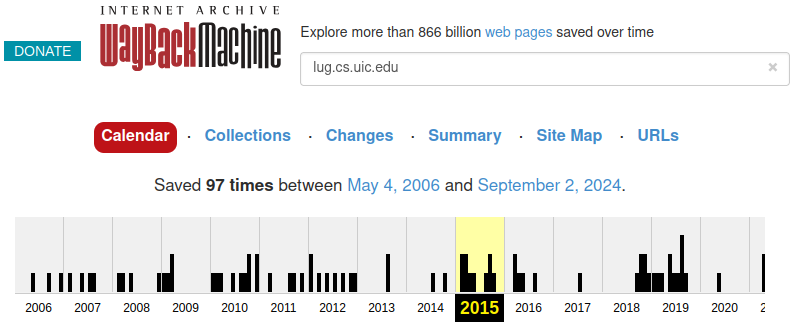
\includegraphics[width=0.60\textwidth]{site_history.png}
				\caption{Our website has been active since 2006!}
			\end{figure}
			\pause
		\item We share an office with ACM in \underline{SELE 2264}
			where \textit{anyone} can come in and talk technology!
			\pause
		\item We maintain one of the largest CS org Discord servers,
			nearing \textbf{500} members :D
	\end{itemize}
\end{frame}

\subsection{Meet the Officers}
\begin{frame}{Meet the Officers}
	{\Huge President}
	\begin{columns}
		\begin{column}{0.5\textwidth}
			\begin{itemize}
				\item {\Large Ethan Wong}
				\item Contact:
					\href{mailto:ewong25@uic.edu}{\texttt{ewong25@uic.edu}}
				\item Maintaining LUG since 2024
				\begin{itemize}
					\item Distro: Arch
					\item Owns \textit{too many} Thinkpads
					\item Loves homelabbing and enterprise rack-servers
					\item Interested in VR hardware
				\end{itemize}
			\end{itemize}
		\end{column}
		\begin{column}{0.5\textwidth}
			\begin{figure}
				\centering
				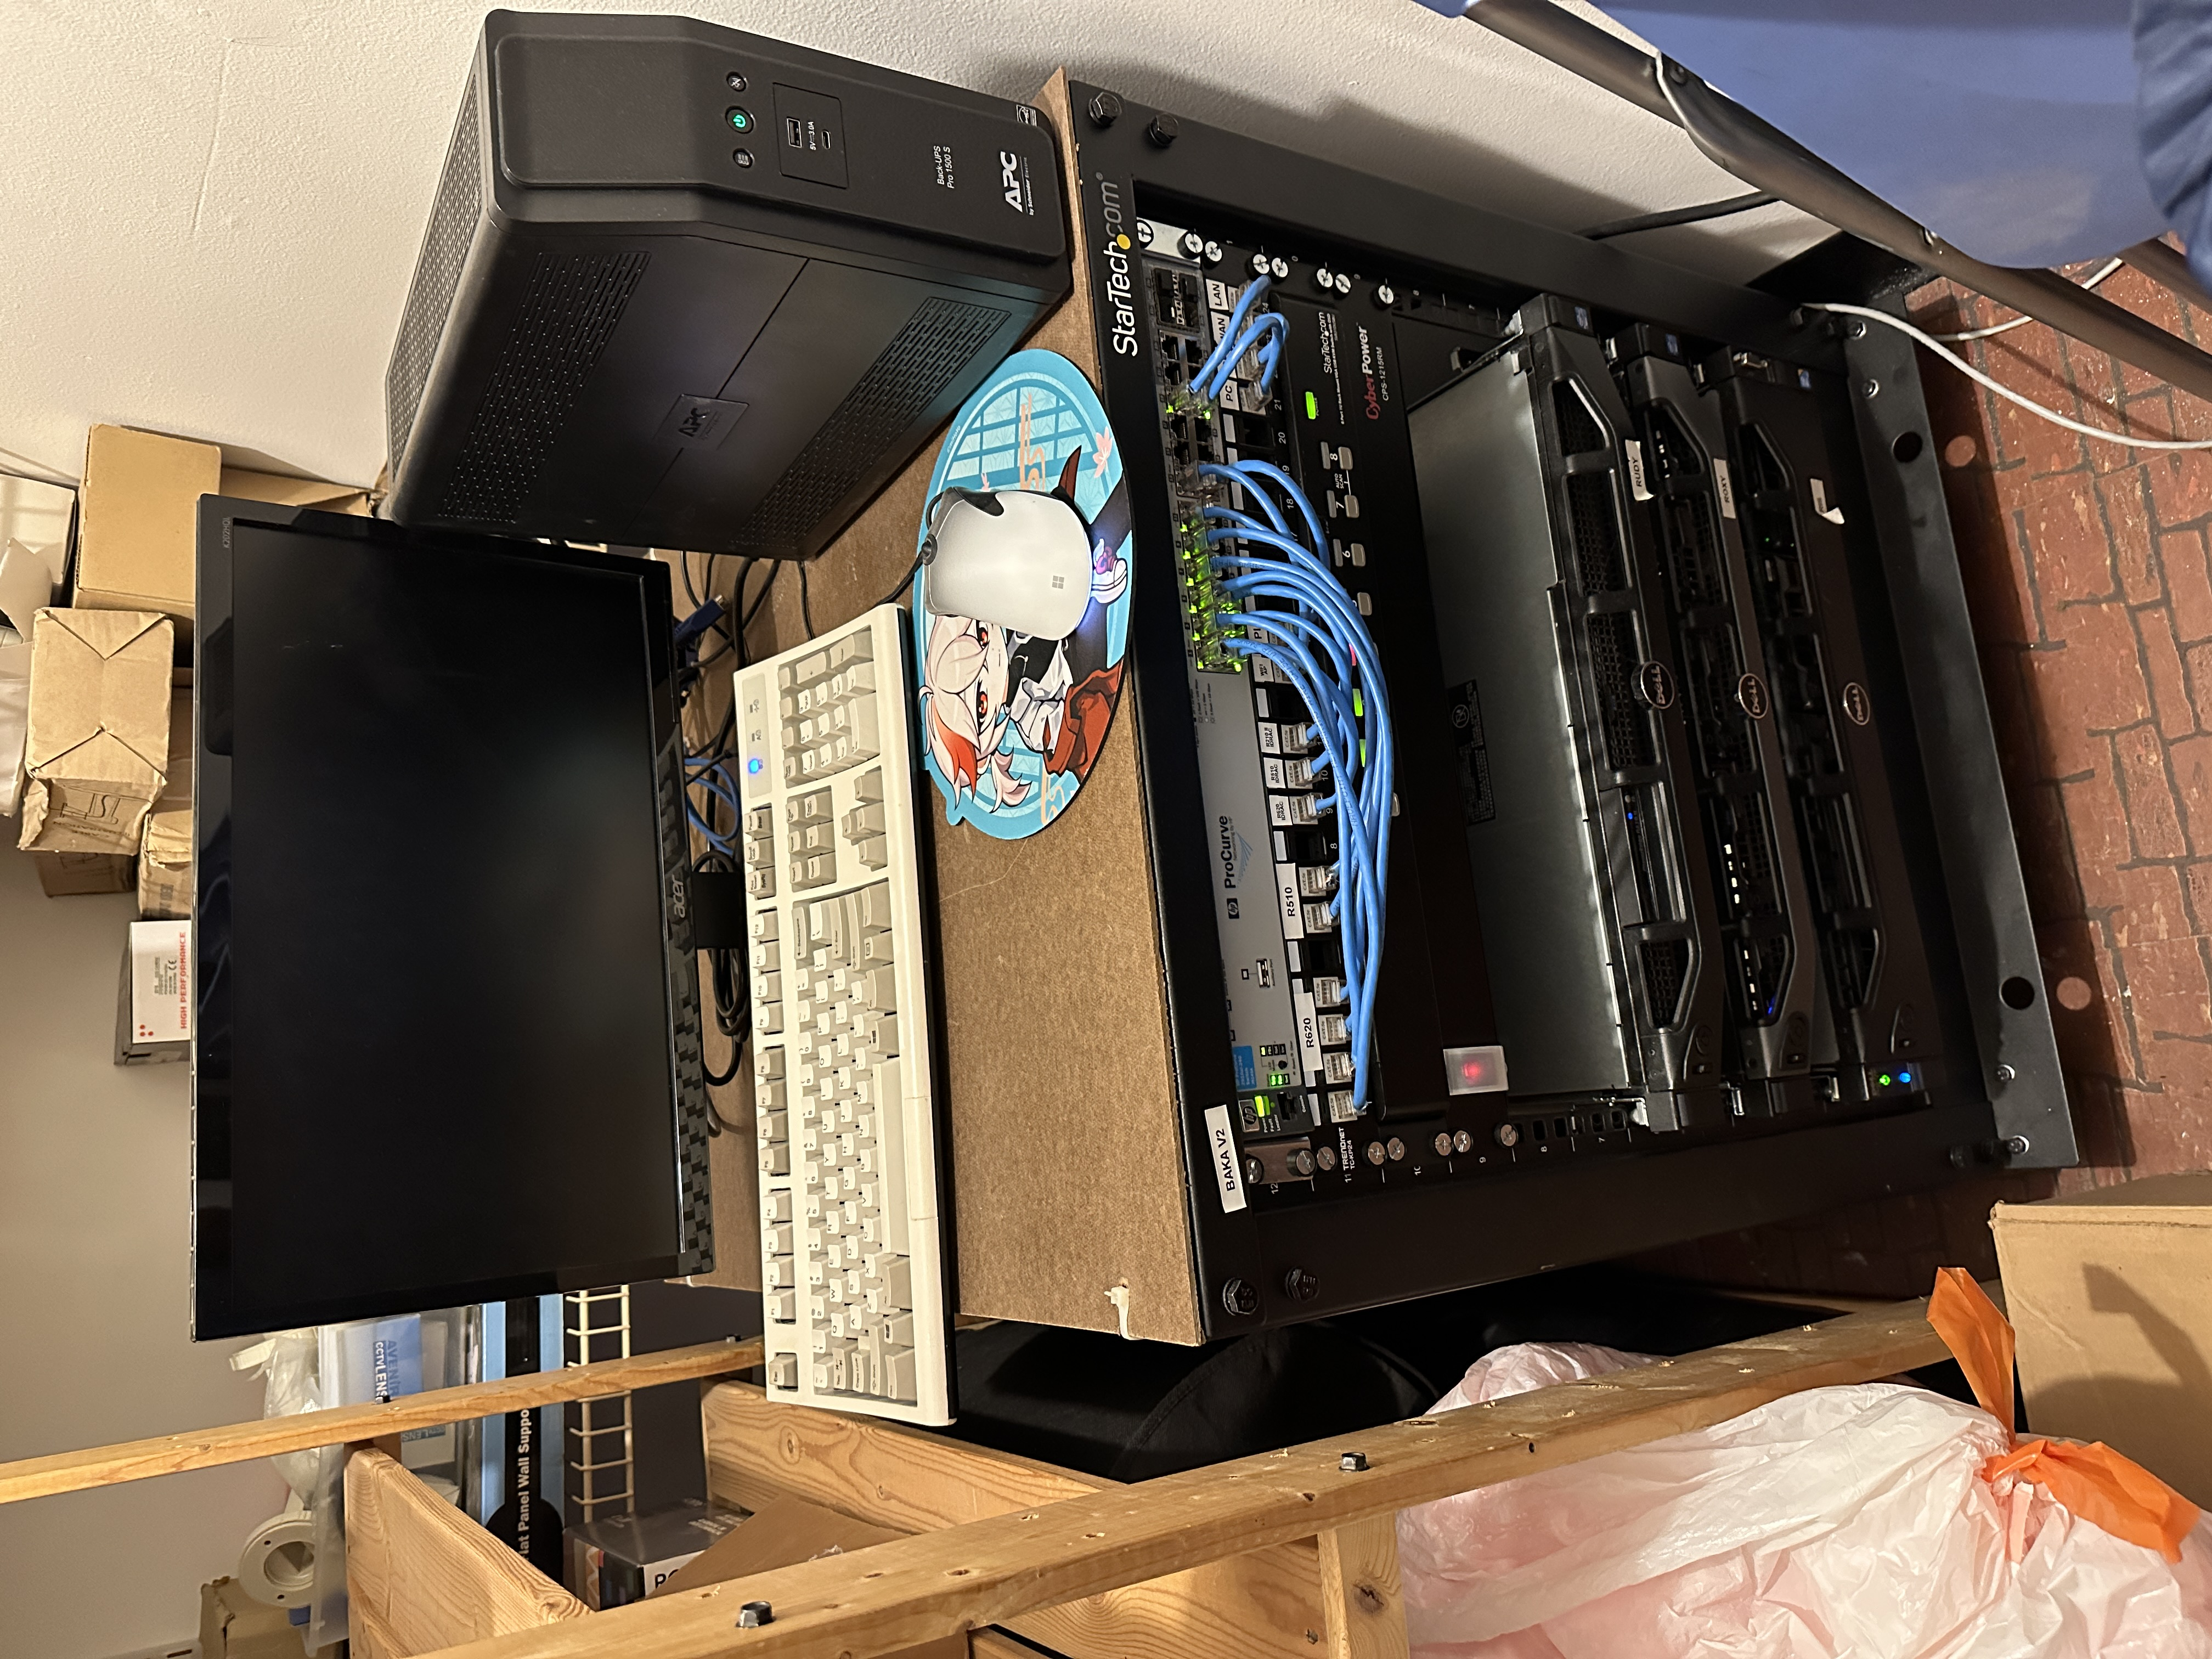
\includegraphics[width=0.9\textwidth,angle=270]{neko-homelab.jpg}
				\caption{My Homelab}
			\end{figure}
		\end{column}
	\end{columns}
\end{frame}

\begin{frame}{Meet the Officers}
	{\Huge Vice President}
	\begin{columns}
		\begin{column}{0.5\textwidth}
			\begin{itemize}
				\item {\Large Jacob Cohen}
				\item Contact:
					\href{mailto:jcohen30@uic.edu}{\texttt{jcohen30@uic.edu}}
				\item Maintaining LUG since 2024
				\begin{itemize}
					\item Uses Debian on home server
					\item PhD Student under Professor Eriksson
					\item Runs ACM's SIG Systems
				\end{itemize}
			\end{itemize}
		\end{column}
		% \begin{column}{0.50\textwidth}
		% 	\begin{figure}
		% 		\centering
		% 		\includegraphics[width=\textwidth,angle=270]{jcohen30.jpg}
		% 	\end{figure}
		% \end{column}
	\end{columns}
\end{frame}

\begin{frame}{Meet the Officers}
	{\Huge Treasurer}
	\begin{columns}
		\begin{column}{0.5\textwidth}
			\begin{itemize}
				\item {\Large Kevin Cordero}
				\item Contact:
					\href{mailto:kcord2@uic.edu}{\texttt{kcord2@uic.edu}}
				\item Maintaining LUG since 2021
				\begin{itemize}
					\item Distro: Linux Mint
					\item Has a website \url{https://olympicene.dev/}
					\item Loves movies!
					\item Also has a homelab (Dell Poweredge R320)
				\end{itemize}
			\end{itemize}
		\end{column}
		% \begin{column}{0.50\textwidth}
		% 	\begin{figure}
		% 		\centering
		% 		\includegraphics[width=\textwidth,angle=270]{kcord2.jpg}
		% 	\end{figure}
		% \end{column}
	\end{columns}
\end{frame}

\begin{frame}{Contact Us}
	\Huge Email us! \href{mailto:lug-officers@uic.edu}{\texttt{lug-officers@uic.edu}}
\end{frame}

\section{What's Linux?}
\begin{frame}{Table of Contents}
	\tableofcontents[currentsection]
\end{frame}

\begin{frame}{What's Linux?}
	\begin{columns}
		\begin{column}{0.5\textwidth}
			\textbf{Linux} is a free and open-source operating
			system kernel. Linux is part of a family of operating
			systems that bundle various pieces of software to form
			a complete OS, called \underline{Linux distros}.
		\end{column}
		\begin{column}{0.5\textwidth}
			\begin{figure}
				\centering
				\includesvg[width=0.9\textwidth]{tux.svg}
				\caption{Tux, the Linux mascot}
			\end{figure}
		\end{column}
	\end{columns}
\end{frame}

\begin{frame}{Why Linux?}
	\begin{itemize}
		\item It's truly free!
			\pause
			\begin{itemize}
				\item Anyone can view, modify, and redistribute
					the the kernel and its underlying
					source code.
					\pause
				\item It's actually libre/available for no
					charge.\footnote{most of the time}
					\pause
			\end{itemize}
		\item Linux powers millions of devices like Android
			smartphones, Chromebooks, and even the \textbf{top 500}
			supercomputers in the world!
		\item Unix-like systems like Linux are widespread in academia.
			Learning its usage is beneficial to your research and
			coursework!
			\pause
		\item Linux systems are tailored to software development,
			programming and installing dependencies is far easier
			on Linux than other operating systems.
			\pause
		\item It's \underline{not} Windows.
			\pause
			\begin{itemize}
				\item Or macOS either...
			\end{itemize}
			\pause
	\end{itemize}
	Curious? Check out our Linux Week event coming soon!\footnote{will be
	announced later in the presentation}
\end{frame}

\section{What We've Been Up To}
\begin{frame}{Table of Contents}
	\tableofcontents[currentsection]
\end{frame}

\begin{frame}{Past Presentations}
	In the past, we've ran presentations/workshops on various topics to
	spread knowledge of how to better use a Linux system. Some of these include:
	\pause
	\begin{itemize}
		\item Vim, the ubiquitous text editor
			\pause
		\item SystemD, the system and service manager
			\pause
		\item Makefiles
			\pause
		\item GDB
			\pause
		\item \textit{and more...}
			\pause
	\end{itemize}
	You may have even encountered these in your coursework!
\end{frame}

\begin{frame}{Website}
	\begin{columns}
		\begin{column}{0.4\textwidth}
			\begin{figure}
				\centering
				
\includegraphics[width=\textwidth]{website.png}
				\caption{LUG Website}
			\end{figure}
		\end{column}
		\begin{column}{0.6\textwidth}
			We've been building a \textit{community-contributed}
			knowledge-base for Linux users at UIC who...
			\pause
			\begin{itemize}
				\item \underline{daily-drive} Linux
				\pause
				\item use Linux in a class (i.e.
					\texttt{systems\{1..4\}.cs.uic.edu})
					\pause
				\item need information about Linux, GNU, Free
					Software, etc. or are otherwise trying
					to learn
					\pause
			\end{itemize}
			Our new website has been in active development since
			\textbf{2022}. Students are also free to contribute,
			our website is open source under the MIT license. Check
			it out! \url{https://lug.cs.uic.edu}
		\end{column}
	\end{columns}
\end{frame}

\begin{frame}{Projects}
	We've been working on fun things within the ACM/LUG room, mostly
	hobbyist projects that \textit{anyone} can get involved with!
	\pause
	\begin{figure}
		\centering
		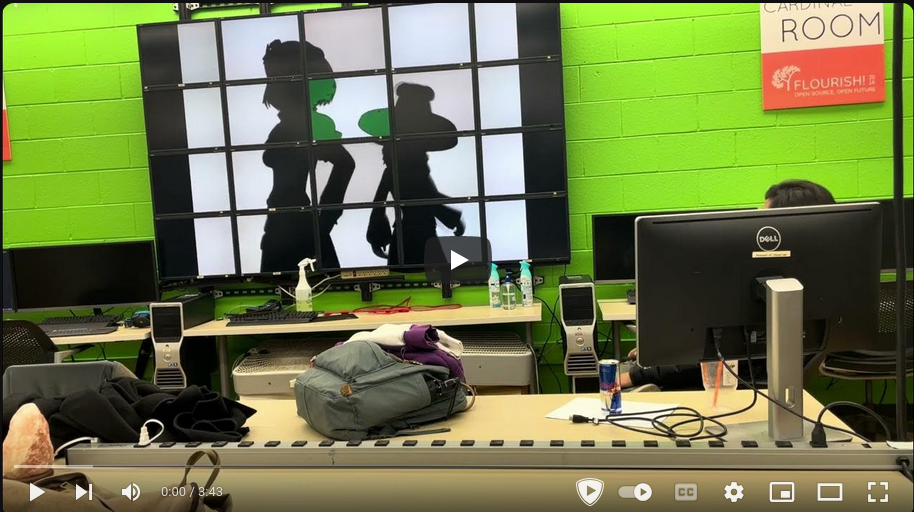
\includegraphics[width=0.60\textwidth]{bad-apple.png}
		\caption{Bad Apple on the Monitor Wall (\url{https://www.youtube.com/watch?v=IMMLflKIPig})}
	\end{figure}
\end{frame}

\begin{frame}{Projects}
	Apart from that, our GitHub has many of our open-source works, including:
	\pause
	\begin{itemize}
		\item Cerberus, an LDAP user management app
			\pause
		\item \texttt{eventfetch}, automated event flyers
			\pause
		\item \texttt{doorkeeper-driver}, an evdev driver for keycard readers
			\pause
		\item \texttt{doorbot}, a Discord bot to keep access in the ACM/LUG office
			\pause
	\end{itemize}
	Among many other incomplete works lost in the weeds due to time. Check it
	out here: \url{https://github.com/lugatuic}.
\end{frame}

\begin{frame}{Server Rack}
	\begin{columns}
		\begin{column}{0.4\textwidth}
			\begin{figure}
				\centering
				\includegraphics[width=0.9\textwidth]{server-rack.jpg}
				\caption{ACM/LUG Server Room}
			\end{figure}
		\end{column}
		\begin{column}{0.6\textwidth}
			We share a server rack with \textbf{ACM}. \pause We own
			our own server on the rack: \texttt{miku}.
			\texttt{miku} is a Dell Poweredge R610 running Proxmox,
			a KVM-based hypervisor which manages virtual machines.
			This server has an overkill amount of hardware.
		\end{column}
	\end{columns}
\end{frame}

\section{Future Plans}
\begin{frame}{Table of Contents}
	\tableofcontents[currentsection]
\end{frame}

\begin{frame}{Tentative Semester Presentations}
	We're proud to offer these topics as workshops this semester.
	\pause
	\begin{itemize}
		\item Linux, Libreboot, and Thinkpads
		\item Intermediate Tmux Usage
		\item Homelabbing
	\end{itemize}
	\pause
	\textit{If you want a specific topic covered or want to present your
	own presentation, let us know!
	\href{mailto:lug-officers@uic.edu}{\texttt{lug-officers@uic.edu}}}
\end{frame}

\begin{frame}{Linux Week}
	Linux Week is our (somewhat) annual event where we teach introductory
	Linux skills to newbies.
	\pause

	Linux Week 2024 is being held \underline{within the next two
	weeks!}\footnote{pending room reservation from the university}
	\pause
	
	Topics include:
	\begin{itemize}
		\item Installing Linux on Your Machine
		\item Coreutils and Filesystem Usage
		\item Package Management
		\item Shell Scripting and Pipelines
		\item Software Freedoms and Copyleft
	\end{itemize}
	\pause

	Keep tabs on our Discord and the newsletter listserv for further
	announcements.
\end{frame}

\begin{frame}{Closing Remarks}
	\begin{center}
		\Huge Thank you!
	\end{center}
\end{frame}

\begin{frame}{Closing Remarks}
	\begin{columns}
		\begin{column}{0.5\textwidth}
			\textbf{Officers}
			\begin{figure}
				\centering
				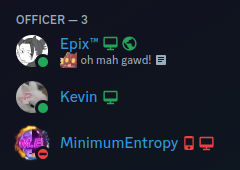
\includegraphics[width=0.60\textwidth]{officers.png}
			\end{figure}
		\end{column}
		\begin{column}{0.5\textwidth}
			The information in this presentation will be made
			available\footnotemark on our website!\\
			\url{https://lug.cs.uic.edu}
			
			\bigskip
			Join our Discord!

			\begin{figure}
				\centering
				\includesvg[width=0.5\textwidth]{lug-discord.svg}
				\caption{\url{https://discord.gg/NgxTR7PX5e}}
			\end{figure}
		\end{column}
	\end{columns}

	\footnotetext{sooner or later}
\end{frame}

\end{document}

% vim: set tw=80 ts=4 sw
